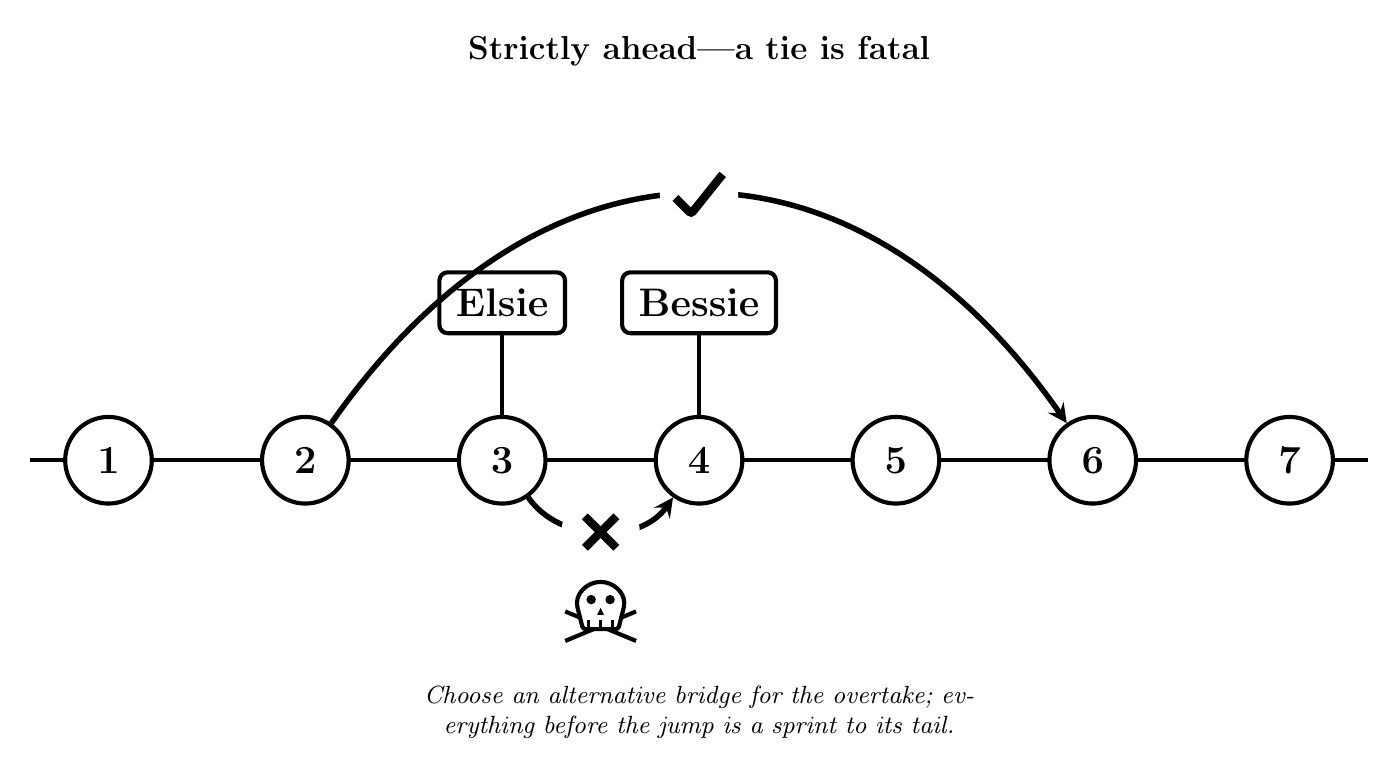
\begin{tikzpicture}[
    >=stealth,
    island/.style={circle, draw, line width=1.5pt, fill=white, minimum size=1.1cm, font=\Large\bfseries},
    character/.style={draw=black, fill=white, line width=1.5pt, rounded corners=3pt, inner sep=6pt, font=\Large\bfseries}
]

\tikzset{
  skull/.pic={
    % crossbones
    \draw[line width=1.5pt, rounded corners=0.5pt] (-0.3, -0.3) -- (0.3, -0.05);
    \draw[line width=1.5pt, rounded corners=0.5pt] (-0.3, -0.05) -- (0.3, -0.3);
    % skull background
    \fill[white] (-0.2, 0) arc (180:0:0.2) -- (0.15,-0.2) -- (-0.15,-0.2) -- cycle;
    \draw[line width=1.5pt, rounded corners=1pt] (-0.2, 0) arc (180:0:0.2) -- (0.15,-0.2) -- (-0.15,-0.2) -- cycle;
    \fill (-0.08, 0.05) circle (0.04);
    \fill (0.08, 0.05) circle (0.04);
    \fill (0,-0.02) -- (-0.03, -0.08) -- (0.03, -0.08) -- cycle;
    \draw[line width=1pt] (-0.1, -0.2) -- (-0.1, -0.12);
    \draw[line width=1pt] (0, -0.2) -- (0, -0.12);
    \draw[line width=1pt] (0.1, -0.2) -- (0.1, -0.12);
  },
  checkmark/.pic={
    \draw[line width=3pt, rounded corners=1pt] (-0.3,-0.05) -- (-0.1,-0.25) -- (0.3,0.25);
  },
  crossmark/.pic={
    \draw[line width=3pt, rounded corners=1pt] (-0.2,-0.2) -- (0.2,0.2);
    \draw[line width=3pt, rounded corners=1pt] (-0.2,0.2) -- (0.2,-0.2);
  }
}

\gid{islands}{
    \draw[line width=1.5pt] (1.5, 0) -- (18.5, 0);
    \foreach \i in {1,...,7} {
        \node[island] (n\i) at (\i*2.5, 0) {\i};
    }
}

\gid{bessie}{
    \node[character] (bessie) at (10, 2.0) {Bessie};
    \draw[line width=1.5pt] (bessie.south) -- (n4.north);
}

\gid{elsie}{
    \node[character] (elsie) at (7.5, 2.0) {Elsie};
    \draw[line width=1.5pt] (elsie.south) -- (n3.north);
}

\gid{main-bridge}{
    \draw[->, line width=2pt] (n3) to[bend right=55] 
        node[midway, fill=white, circle, inner sep=10pt] (xnode) {} 
        (n4);
    \pic at (xnode.center) {crossmark};
    \pic[scale=1.5] at ([yshift=-0.4cm]xnode.south) {skull};
}

\gid{alternative-bridge}{
    \draw[->, line width=2pt] (n2) to[out=55, in=125, looseness=1.3] 
        node[midway, fill=white, circle, inner sep=10pt] (checkbg) {} 
        (n6);
    \pic at (checkbg.center) {checkmark};
}


% --- enhancer additions ---
\coordinate (fig-east) at (current bounding box.east);
\coordinate (fig-west) at (current bounding box.west);
\gid{header-1}{\node[anchor=south, font=\bfseries\large, align=center] at ([yshift=14pt]current bounding box.north) {Strictly ahead—a tie is fatal};}
\gid{footer-1}{\node[anchor=north, font=\itshape\small, align=center, text width=10cm] at ([yshift=-12pt]current bounding box.south) {Choose an alternative bridge for the overtake; everything before the jump is a sprint to its tail.};}
\end{tikzpicture}